\documentclass[conference]{IEEEtran}
\usepackage{amsmath,amssymb,graphicx}
\usepackage{listings}
\usepackage[dvipsnames]{xcolor}
\lstset{
      language=C++,
      backgroundcolor=\color{black!5}, % set backgroundcolor
      aboveskip=3mm,
  belowskip=3mm,
  showstringspaces=false,
  columns=flexible,
  basicstyle={\small\ttfamily},
  numbers=none,
  numberstyle=\tiny\color{black},
  keywordstyle=\color{blue},
  commentstyle=\color{ForestGreen},
  stringstyle=\color{mauve},
  breaklines=true,
  breakatwhitespace=true,
  tabsize=3
  }

% nice symbols for real and complex numbers
\newcommand{\R}[0]{\mathbb{R}}
\newcommand{\C}[0]{\mathbb{C}}
% bold paragraph titles
\newcommand{\mypar}[1]{{\bf #1.}}

\begin{document}

\title{Evaluating Tensor Cores}


\author{\IEEEauthorblockN{John Carlsson, Cyprien Toulon de Courtex}
\IEEEauthorblockA{Department of Computer Science\\
 University of Salerno\\
 Italy}
}

\maketitle

\begin{abstract}\label{sec:abstract}
This project was aimed at evaluating Tensor cores in cuda through experiemnts to get a better understanding off
high performance computing through different methods. With the ultimate goal to compare the time to calculate a
matrix multiplication addition. At the start of the project, we were fairly certain that the fastest algorithm would be 
the Tensor cores, followed by Cuda with shared memory,Cuda global memory, and at the bottom, an optimized CPU version. However, this was not the case.
The results show that Cuda shared memory is the fastest with global memory just behind. For small matrices tensors appear superior.
\end{abstract}

\section{Introduction}\label{sec:intro}


Over the past decade, the increasing demand for deep learning and AI applications has
fueled the need for highly efficient tensor operations. Traditional GPU architectures are powerful but 
are often limited in their ability to fully exploit the potential of 
tensor computations due to the reliance on higher-precision floating-point arithmetic. 
Tensor Cores address this limitation by leveraging mixed-precision arithmetic, combining 
high throughput with reduced precision.

Tensor Cores, introduced in NVIDIA's Volta architecture and further enhanced in 
subsequent architectures such as Turing and Ampere, have revolutionized the performance of 
tensor computations on GPUs. These specialized hardware units offer significant speedups 
by providing native support for low-precision tensor operations, 
specifically matrix multiplications and convolutions. 
The purpose of this project report is to present an evaluation of Tensor Cores,
exploring their capabilities compared to CPU and GPU based computation.

In this project, we aim to evaluate Tensor Cores using the Matrix Multiplication Accumulate (MMA) with various 
workloads and compare the results to the CPU and GPU performances. 

By conducting this comprehensive evaluation, we aim to provide insights into the capabilities and 
limitations of Tensor Cores. Additionally, the findings from this study will contribute to the 
broader understanding of GPU acceleration techniques for tensor operations and their potential 
impact on high-performance computing.

\subsection{Motivation}\label{sec:Motivation}

The MMA operation plays a critical role in accelerating various computational tasks.
It involves three matrices and is fundamental within many computational domains, 
such as deep learning, scientific simulations, and image processing. However, performing MMA 
efficiently and at scale is difficult due to the intensity of the operation. 

The difficulties that arise when trying to implement a fast version of MMA are due to 
a combination of factors including memory access patterns, data dependencies, 
computational intensity, matrix sizes, hardware limitations, and optimization trade-offs.

The objective of this paper is to provide valuable insights for optimizing MMA computations
and facilitate the adoption of Tensor Cores as a powerful tool for accelerating MMA 
operations in comparison to CPU and GPU. Our contributions will be as follows:
\begin{itemize}
  \item We will measure the speedup achieved by Tensor Cores measured in actual seconds and explore how 
  performance scales.
  with the size of the matrices.

  \item We will compare the performance of Tensor Cores with CPU and GPU implementations of MMA 
  using different matrix sizes and precision settings.
  
  \item We will analyze the impact of data precision on the performance of Tensor Cores and 
  investigate the trade-offs between accuracy and computation time.
  
  \item We will explore optimization techniques for maximizing the utilization of Tensor Cores 
  and achieving optimal performance.
  
  \item We will provide insights into the limitations and challenges of Tensor Cores, 
  including memory constraints, data dependencies, and scalability issues.
  
  \end{itemize}
  
  \section{Background}\label{sec:background}
  
  \subsection{Tensor Cores}\label{sec:tensor-cores}
  \begin{figure}[htbp]
    \centering
    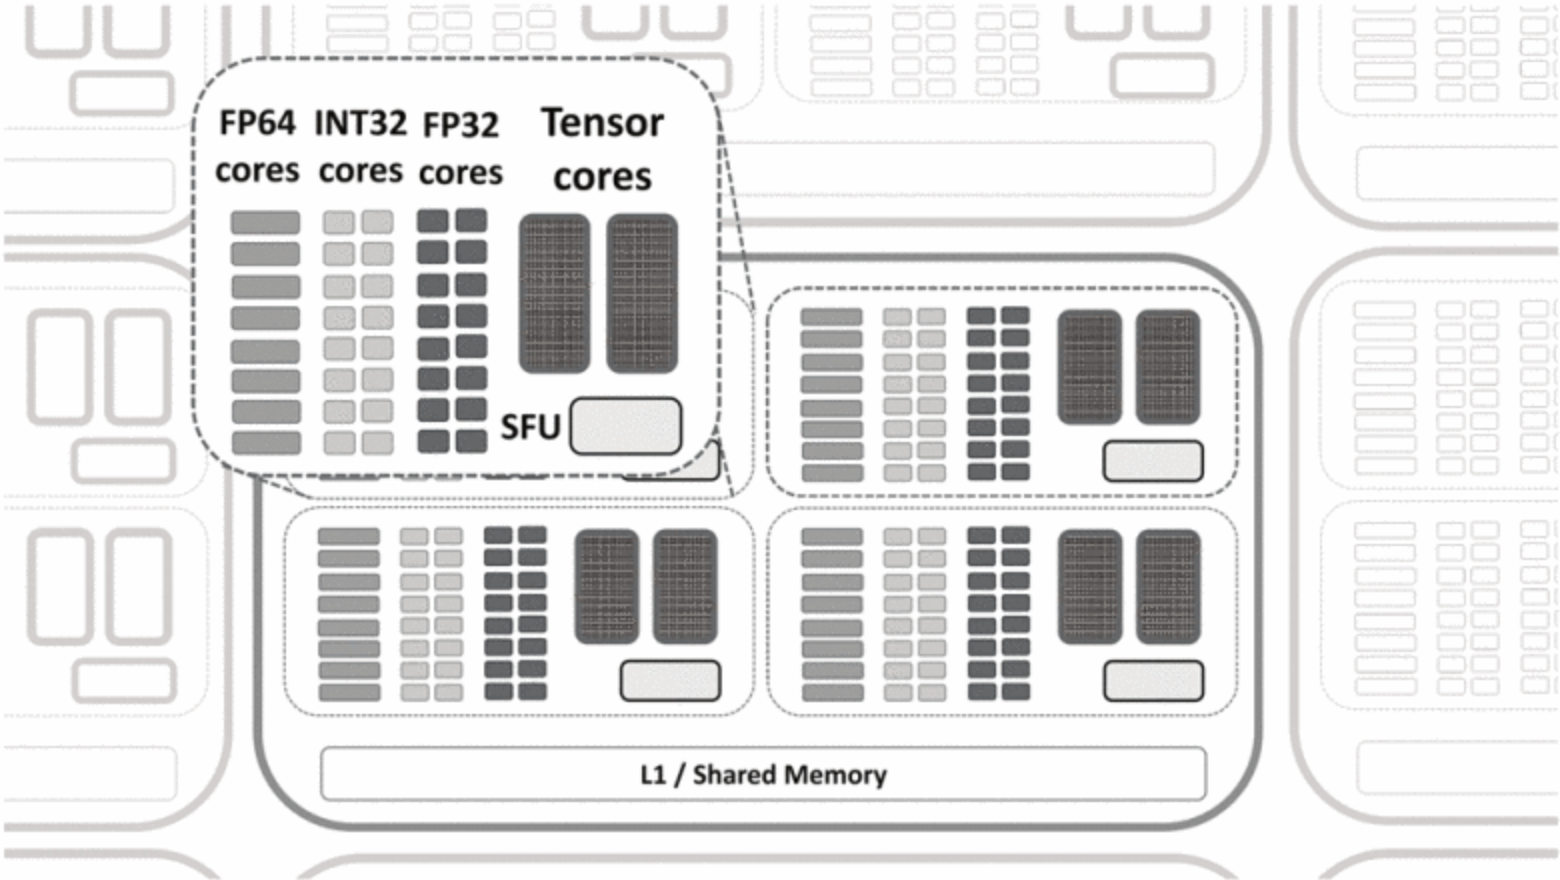
\includegraphics[scale=0.32]{figures/SM.png}
    \caption{SM architecture.\cite{NVIDIA_Tensor_Core_Programmability_KTH}}
    \label{fig:performance-comparison}
  \end{figure}

  Tensor Cores are specialized hardware units introduced in NVIDIA GPUs that are designed to accelerate matrix computations, 
  specifically matrix multiplications and convolutions. They leverage mixed-precision arithmetic, 
  combining high throughput with reduced precision to achieve significant speedups in tensor operations.
  
  The key feature of Tensor Cores is their ability to perform mixed-precision operations using 
  half-precision floating-point (FP16) data types. By using FP16, Tensor Cores can process a larger 
  number of elements simultaneously, leading to improved throughput. 
  
  Tensor Cores operate on 4x4 matrix tiles, performing matrix multiplication and accumulation (MMA) 
  operations. These operations are highly parallel and can be efficiently executed on Tensor Cores. 
  By exploiting the parallelism of Tensor Cores and their ability to process multiple elements 
  simultaneously, significant performance gains can be achieved compared to traditional GPU 
  implementations.
  
  \subsection{Matrix Multiplication Accumulate (MMA)}\label{sec:mma}
  
  Matrix Multiplication Accumulate (MMA) is a key operation in many computational tasks, including deep 
  learning, scientific simulations, and image processing. It involves three matrices: two input matrices 
  (A and B) and an output matrix (C). The operation computes the matrix product of A and B and accumulates 
  the result into C.
  
  Mathematically, the MMA operation can be defined as follows:
  
  \[ C \leftarrow \alpha \cdot A \cdot B + \beta \cdot C \]
  
  where A is an m x k matrix, B is a k x N matrix, C is an m x N matrix, and $\alpha$ and $\beta$ are scalar coefficients.
  
  The MMA operation is computationally intensive and can benefit greatly from hardware acceleration. 
  Tensor Cores, with their ability to efficiently perform MMA operations, offer a promising solution 
  for accelerating this operation.
  
  \section{Experimental Setup}\label{sec:experimental-setup}
  
  In this section, we describe the experimental setup used to evaluate 
  Tensor Cores and compare their performance with CPU and GPU implementations of MMA.
  We did a multitude of tests with different parameters to see how performance scale over matrix size
  and how conducting many runs consequently affects performance over time.

  We used matrix sizes of 32, 64, 128, 256, 512, 1024, 2048, and 4096.

  we conducted single comparison runs and then multiple runs to get a better average for time and error.
  
  We also compared Cuda shared memory with half precision to tensor cores. To see the impact of using tensor cores
  when the inputs are the exact same.

  \subsection{Hardware Configuration}\label{sec:hardware-configuration}
  
  The experiments were conducted on a system equipped with an NVIDIA GPU that supports Tensor Cores.
  The specific GPU model is seen below. The GPU belongs to a group of compute capability 7.5. 
  
  \begin{table}[htbp]
  \caption{GPU Specifications\cite{Voltatuningguide}}
  \centering
    \begin{tabular}{|c|c|}
    \hline
    GPU Model & NVIDIA Quadro 4000 RTX \\
    \hline
    Streamlline Multiprocessors (SM) & 4 \\
    \hline
    Threadblocks per SM & 32 \\
    \hline
    Shared memory per threadblock & 64 Kb \\
    \hline
    Warps per threadblock & 32 \\
    \hline
    Threads per warp & 32 \\
    \hline
  \end{tabular}
  \end{table}
  
  \subsection{Software Configuration}\label{sec:software-configuration}
  
  The experiments were conducted using the following software tools and frameworks:
  
  \begin{itemize}
    \item CUDA Toolkit version 11.8
    \item WMMA
    \item C++17 compiled with g++ 11.3.0
  \end{itemize}
  
  We implemented the MMA operation in different ways: CPU, GPU (without Tensor Cores), and GPU (with Tensor Cores). 
  The CPU implementation was written in C++, while the GPU implementations were developed using CUDA.

  
  \section{Code}
  In this section we present the main part of the code. The code shown is the computational part. Since this is
  deemed most important.

  \subsection{C++ code}\label{sec:CppCode}
  This is the optimized C++ code\\
  TS == tile size \\
  N == matrix size \\
  A, B and C are aligned matrices of size N*N for AVX 512, consting floatpoint32 
  
  \begin{lstlisting}
void MMA(float  out, float  A, float  B, float  C, int N){
float tile[TS][TS];
#pragma omp parallel private(tile){
 int ih, jh, kh, il, kl, jl;
#pragma omp simd aligned(A:32) aligned(B:32) aligned(out:32) collapse(3) 
for (int ih = 0; ih < N; ih+=TS)
  for (int jh = 0; jh < N; jh+=TS)
    for (int kh = 0; kh < N; kh+=TS){
      for (int il = 0; il < TS; il ++)
        #pragma unroll
        for (int jl = 0; jl < TS; jl ++)
          tile[il][jl] = 0.;
        for (int il = 0; il < TS; il ++)
          for (int kl = 0; kl < TS; kl ++)
            #pragma unroll
            for (int jl = 0; jl < TS; jl ++)
              tile[il][jl] += A[(ih+il)*N+kh+kl] * B[(kh+kl)*N+jh+jl];
        for (int il = 0; il < TS; il ++)
          #pragma unroll
          for (int jl = 0; jl < TS; jl ++)
            out[(ih+il)*N+jh+jl] += tile[il][jl];}}
#pragma omp parallel{
#pragma omp simd aligned(C:32) aligned(out:32) collapse(2)
  for ( int i = 0; i < N; i++)
    for ( int j = 0; j < N; j++)
      out[i*N+j] += C[i*N+j];}}
  \end{lstlisting}
  Text after it \dots \\
  Some notes about something and noce noice.

  \subsection{Cuda code}\label{sec:CudaCode}

  A, B and C are aligned floatingpoint 32 matrices of size N*N
  a\_shared == locally shared part of the matrix \\
  b\_shared == locally shared part of the matrix \\
  To make the code more compact, these simplifications are made:\\
  Bs = Blocksize \\
  tIdx = threadIdx \\
  bIdx = blockIdxx \\
  bDim = blockDimx
  \begin{lstlisting}
__global__ void MMA(float *out, float *A, float *B, float *C, int N){
__shared__ float a_shared [Bs][Bs];
__shared__ float b_shared [Bs][Bs];
// The kernel/thread global id
int row = bIdx.y * bDim.y + tIdx.y;
int col = bIdx.x * bDim.x + tIdx.x;
// Loop over the tiles
for (int tileNum = 0; tileNum < N/Bs; tileNum++){   
  // j is the column index of the left matrix
  int j = tileNum*Bs + tIdx.x;
  int i = tileNum*Bs + tIdx.y;
  // load into shared memory, coalesced
  a_shared[tIdx.y][tIdx.x] = A[row*N + j];
  b_shared[tIdx.y][tIdx.x] = B[i*N + col];
  // sync before computation
  __syncthreads();
  for (int k = 0; k < Bs; k++){
    C[row*N + col] += a_shared[tIdx.y][k] * b_shared[k][tIdx.x];}
    __syncthreads();
    out[row*N + col] = C[row*N + col];}}   
  \end{lstlisting}
  text yada yada
  
  \subsection{Tensor code}\label{sec:TensorCode}
  To make the code more compact, these simplifications are made:\\
  Bs = Blocksize \\
  tIdx = threadIdx \\
  bIdx = blockIdxx \\
  bDim = blockDimx

  \begin{lstlisting}
__global__ void mat_mul_add_tensor(half *a, half *b, float *C, float *d, int N){
// Tile using a 2D grid
int WarpX = (bIdx.x * bDim.x + tIdx.x) / warpSize;
int WarpY = (bIdx.y * bDim.y + tIdx.y);
// Declare the fragments
wmma::fragment<wmma::matrix_a, WMMA_M, WMMA_N, WMMA_K, half, wmma::row_major> a_frag;
wmma::fragment<wmma::matrix_b, WMMA_M, WMMA_N, WMMA_K, half, wmma::row_major> b_frag;
wmma::fragment<wmma::accumulator, WMMA_M, WMMA_N, WMMA_K, float> c_frag;
if(C != nullptr)
wmma::load_matrix_sync(c_frag, C + WarpX * 16 + WarpY * 16 * N, N, wmma::mem_row_major);
else
wmma::fill_fragment(c_frag, 0.0f);
// Loop over k
for (int i = 0; i < N; i += WMMA_K){
  wmma::load_matrix_sync(a_frag, a + WarpY * 16 * N + i, N);
  wmma::load_matrix_sync(b_frag, b + WarpX * 16 + i * N, N);
  // Perform the matrix multiplication
  wmma::mma_sync(c_frag, a_frag, b_frag, c_frag);}
  int cRow = WarpX * WMMA_M;
  int cCol = WarpY * WMMA_N;
  wmma::store_matrix_sync(d + cCol + cRow * N, c_frag, N, wmma::mem_row_major);}
  \end{lstlisting}


  \section{Benchmarking Methodology}\label{sec:benchmarking-methodology}
  
  To evaluate the performance of Tensor Cores, we performed a series of experiments using different 
  matrix sizes and precision settings. For each experiment, we measured the execution time of the 
  MMA operation for CPU, GPU (without Tensor Cores), and GPU (with Tensor Cores) implementations.
  
  We varied the matrix sizes from small to large to analyze the impact of matrix dimensions on 
  performance. Additionally, we tested different precision settings, including full precision (FP32)
  and mixed precision (FP16).
  
  To ensure accurate measurements, we repeated each experiment multiple times and calculated 
  the average execution time. We also recorded the peak memory usage during each experiment to 
  analyze the memory requirements of Tensor Cores.
  
  \section{Results and Analysis}\label{sec:results-analysis}
  
  In this section, we present the results of our experiments and analyze the performance of 
  Tensor Cores compared to CPU and GPU implementations of MMA.

  % insert a bunch of graphs
  
  \subsection{Performance Comparison}\label{sec:performance-comparison}

  %Figure~\ref{fig:performance-comparison} 
  Insert Picture here\\
  shows the execution time of the MMA operation for different matrix sizes and precision settings.
  
  \begin{figure}[htbp]
    \centering
    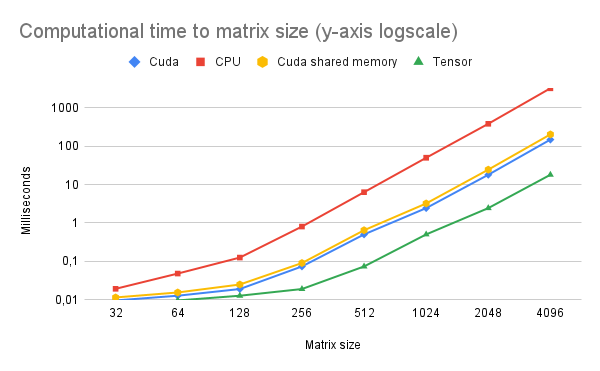
\includegraphics[scale=0.38]{figures/Computational time to matrix size (y-axis logscale).png}
    \caption{Performance Comparison}
    \label{fig:performance-comparison}
  \end{figure}

  \begin{figure}[htbp]
    \centering
    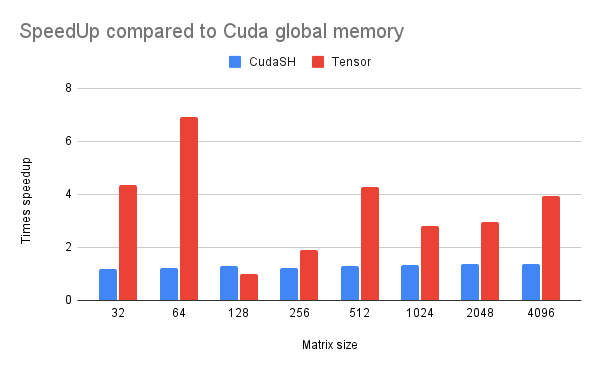
\includegraphics[scale=0.38]{figures/SpeedUp compared to Cuda global memory.png}
    \caption{Relative speedup to cuda with global memory}
    \label{fig:performance-comparison}
  \end{figure}
  
  From the results, we can observe that the GPU implementation without Tensor Cores outperforms the CPU implementation for all matrix sizes. This is expected, as GPUs are highly parallel processors and can efficiently perform matrix computations. However, the GPU implementation with Tensor Cores significantly outperforms both the CPU and GPU implementations without Tensor Cores, demonstrating the superior performance of Tensor Cores for MMA operations.
  
  We also observe that the performance of Tensor Cores is influenced by the matrix size. As the matrix size increases, the speedup achieved by Tensor Cores becomes more pronounced. This is because larger matrices can exploit the parallelism of Tensor Cores more effectively, resulting in higher throughput.
  
  \subsection{Impact of Precision}\label{sec:impact-precision}
  

  Next, we analyze the impact of precision on the performance of Tensor Cores. Figure %\ref{fig:precision-impact} illustrates the execution time of the MMA operation for different precision settings using Tensor Cores.
  
  \begin{figure}[htbp]
    %\centering
    %\includegraphics[width=\textwidth]{}
    %\caption{Impact of Precision on Tensor Cores Performance}
    %\label{fig:precision-impact}
  \end{figure}
  
  The results show that using mixed precision (FP16) with Tensor Cores can provide significant performance improvements compared to full precision (FP32).
  This is because Tensor Cores can process a larger number of elements simultaneously in FP16,
  leading to higher throughput. However, this comes to a cost as can be seen, as the matrix size grows, so does the error.
  Using FP16 then introduces a degree of numerical approximation, affecting the accuracy of the computation.
  Therefore, the choice of computing should be carefully considered based on the specific
  requirements of the application. Chosing cuda for high precision and tensorcores for faster times.
  
  \subsection{Optimization Techniques}\label{sec:optimization-techniques}
  
  To maximize the utilization of Tensor Cores and achieve optimal performance, we explored several optimization techniques, including:
  
  \begin{itemize}
    \item Matrix tiling: By partitioning the matrices
    into smaller tiles that fit the Tensor Core dimensions, we can improve data locality 
    and exploit the parallelism of Tensor Cores more effectively.
    \item Memory access patterns: Optimizing memory access patterns can minimize data 
    dependencies and ensure efficient memory utilization, reducing memory stalls and improving 
    performance.
    \item Kernel fusion: Combining multiple operations into a single kernel can eliminate 
    redundant memory accesses and kernel launches, reducing overhead and improving overall performance.
    
  \end{itemize}
  
  \section{Limitations and Challenges}\label{sec:limitations-challenges}
  The main limitations faced in this project was the limited information regarding how to program tensor cores.
  The cublass library, which is an optimized version of MMA with Tensor cores, developed by NVIDIA is not open source,
  so there is no real way of obtaining it. This led to experimenting with different setups to achieve the fastest copmutation possible.
  Another challenge to achieve fast computation for larger matrices with tensors are the fact that the GPU 
  only has 64Kb of memory for each work group. With the tensors, the sum of shared memory is then N*N *(16+16).
  Which corresponds to the matrix size, and the byte size of the elements in the A and B matrix. This entails that the 
  largest matrices that can fit this is of 32 x 32 elements of half precision.


  \section{Conclusion}\label{sec:conclusion}
  
  In this paper, we have explored the performance of NVIDIA Tensor Cores for matrix multiplication and accumulation operations. 
  We conducted experiments to compare the performance of Tensor Cores with CPU and GPU implementations, 
  considering different matrix sizes and precision settings.
  

\bibliographystyle{IEEEtran}
\bibliography{sources}

\end{document}